\subsection{Potencial Gaussiano}

Em geral, para os ensembles gaussianos estaremos interessados no potencial quadrado, salvo uma escala

\[
	V(x) = x^2
\]

Para estes ensembles vale o clássico resultado da medida de equilíbrio dada pela Lei do Semi-Círculo de Wigner. Se expressa,

\[
\supp \mu_V = [-\sqrt{2}, \sqrt{2}], \frac{d \mu_V}{dx}(x) = \frac{1}{\pi} \sqrt{2 - x^2} 
\]

e teremos das simulações para os três ensembles e suas distribuições esperadas em \ref{fig: semicircle}.

\begin{figure}[ht!]
	\centering
	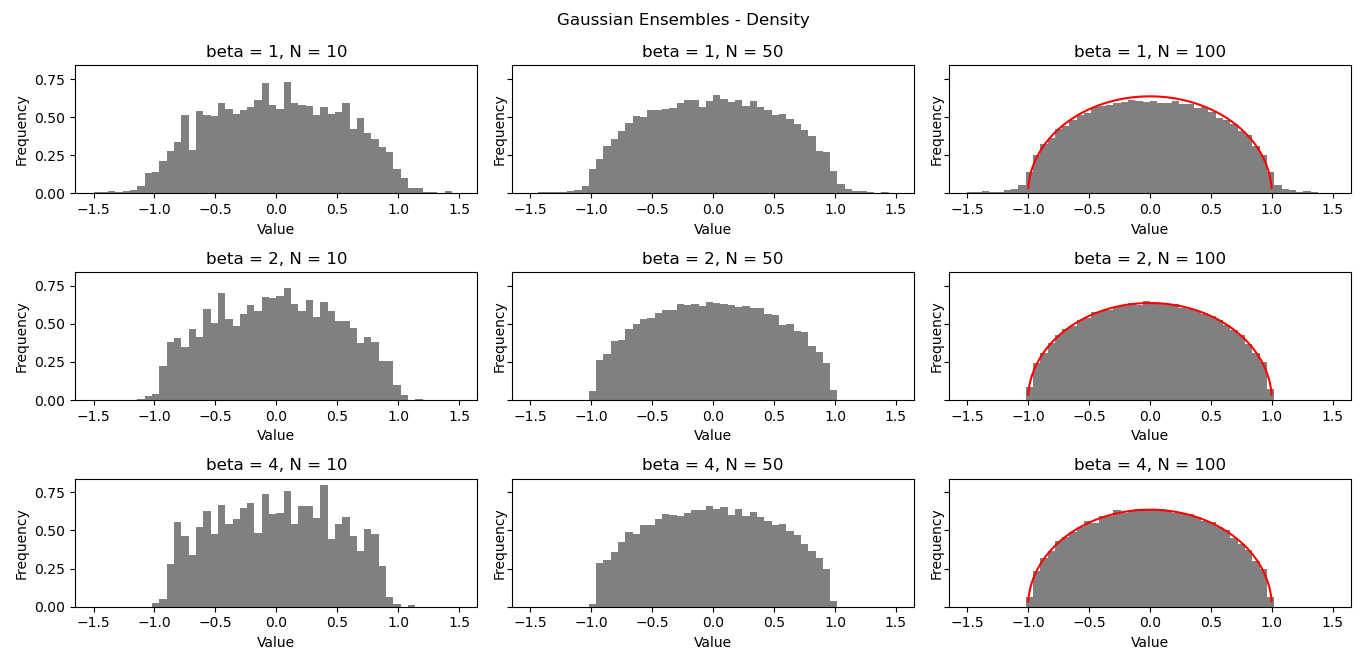
\includegraphics[scale=0.45]{Assets/validationArticleAlg}
	\caption{Validação para ensembles clássicos, utilizamos $200000$ passos registrando a cada $500$ a partir da metade dos passos. $\Delta t = 0.1$, $\gamma = 1$, $\alpha = 1.0$. Para replicar a semente foi $987991650$.}
	\label{fig: semicircle}
\end{figure}

Podemos considerar agora exemplos de potenciais que podem ser aplicados. Lembre que isso implica que nossa entradas são correlacionadas, os ensembles de matrizes para este caso não são tão diretos quanto para entradas independentes. Consideraremos para os exemplos $\beta = 2$. As explicações para os resultados gráficos são retomados na seção sobre as simulações implementadas.


\subsection{Potencial Mônico}

Considere o potencial

\[
	V(x) = \frac{t}{2\alpha} x^{2\alpha}
\]

Onde $t > 0$ é escala e $\alpha \in \Z$. A medida de equilíbrio para $\alpha = 1$ é o semi-círculo de podemos validar na figura com a distribuição em vermelho. De qualquer forma, podemos observar os resultados das simulações para este potencial e notar o comportamento esperado e a distribuição teórica em vermelho para o semicírculo \ref{fig: monic}.


\begin{figure}[ht!]
	\centering
	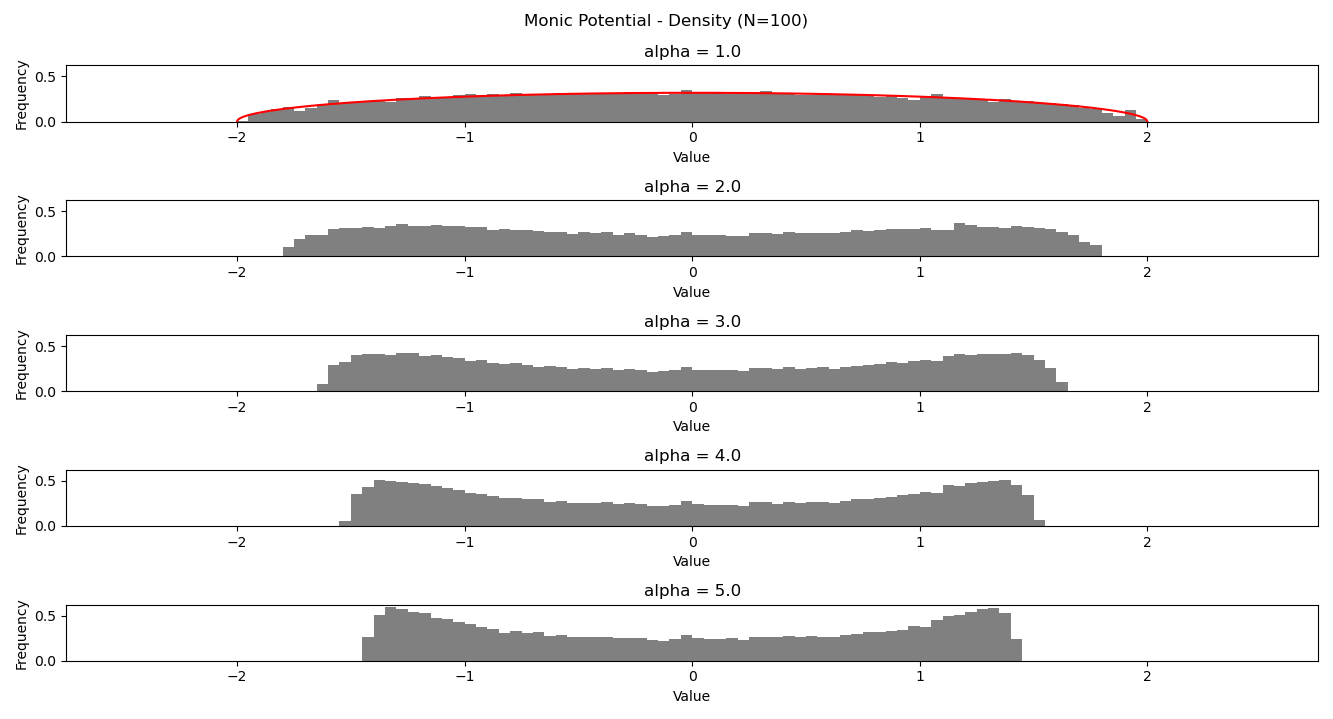
\includegraphics[scale=0.45]{Assets/validationArticleMonic}
	\caption{Validação para potencial mônico, $V(x) = \frac{t}{2 \alpha} x^{2\alpha}$. Utilizamos $1000000$ passos registrando a cada $500$ a partir da metade dos passos. $t = 1$, $\Delta t = 0.1$, $\gamma = 10$, $\alpha = 0.1$. Para replicar a semente foi $987991650$.}
	\label{fig: monic}
\end{figure}


\subsection{Potencial Quártico}

Considere o potencial

\[
	V(x) = \frac{x^4}{4} + t \frac{x^2}{2}
\]

Aqui observaremos pela primeira vez uma transição de estado. Teremos um ponto crítico em $t=-2$ onde a medida se para em dois intervalos $[-b_t, -a_t]$ e $[a_t, b_t]$. Ou seja:

\begin{itemize}
	\item t > -2
	\[
	\supp \mu_V = [-b_t, b_t], \frac{d \mu_V}{dx}(x) = \frac{1}{2\pi} (x^2 - c_t^2) \sqrt{b_t^2 - x^2} 
	\]
	
	com
	
	\[
		c_t^2 \deff\frac{1}{2} b_t^2 + t \deff \frac{1}{3} (-2t + 2 \sqrt{t^2 + 12})
	\]
	
	\item t < -2
	\[
	\supp \mu_V = [-b_t, -a_t] \cup [a_t, b_t], \frac{d \mu_V}{dx}(x) = \frac{1}{2\pi} |x| \sqrt{(x^2 - a_t^2)(b_t^2 - x^2)} 
	\]
	
	com
	
	\[
	a_t \deff \sqrt{-2-t}, b_t \deff \sqrt{2-t}
	\]
\end{itemize}

Observamos o comportamento esperado e a distribuição teórica em vermelho em \ref{fig: quartic}. 


\begin{figure}[ht!]
	\centering
		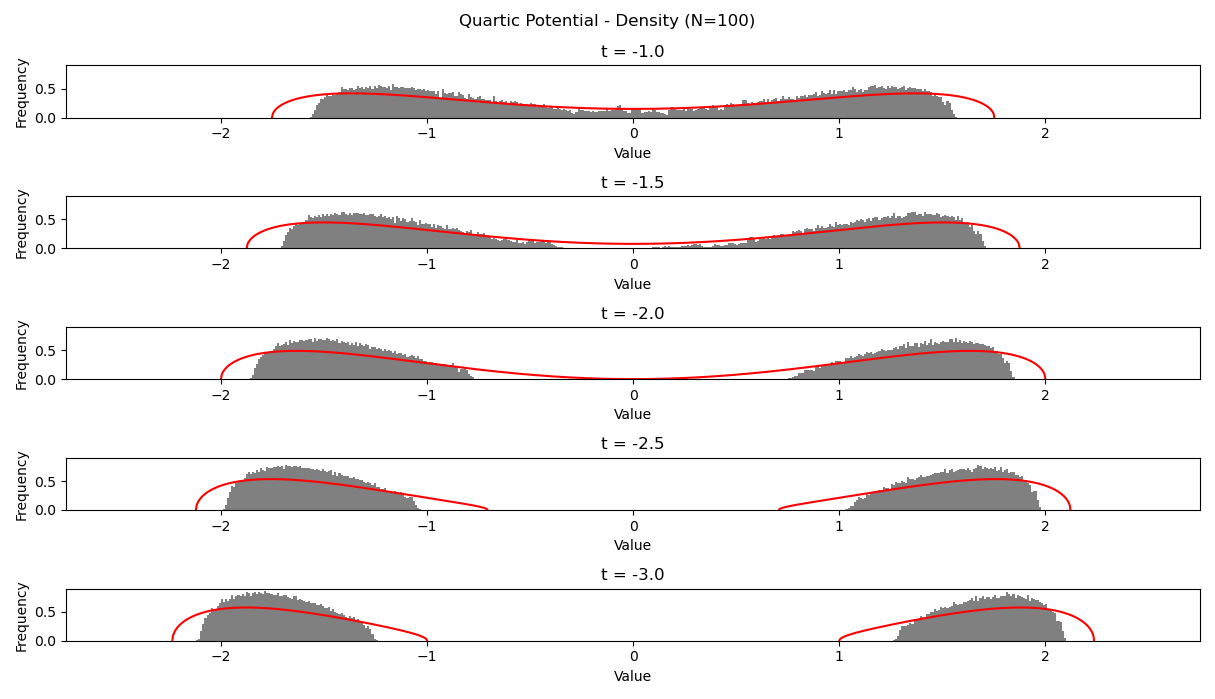
\includegraphics[scale=0.5]{Assets/validationArticleQuartic}
		\caption{Validação para potencial quártico, $V(x) = \frac{1}{4} x^4 + \frac{1}{2} x^2$. Utilizamos $1000000$ passos registrando a cada $500$ a partir da metade dos passos. $\Delta t = 0.1$, $\gamma = 10$, $\alpha = 0.1$. Para replicar a semente usada é $987991650$.}
		\label{fig: quartic}
\end{figure}

